% !TEX root = template.tex

\section{Concluding Remarks}
\label{sec:conclusions}

\begin{figure}
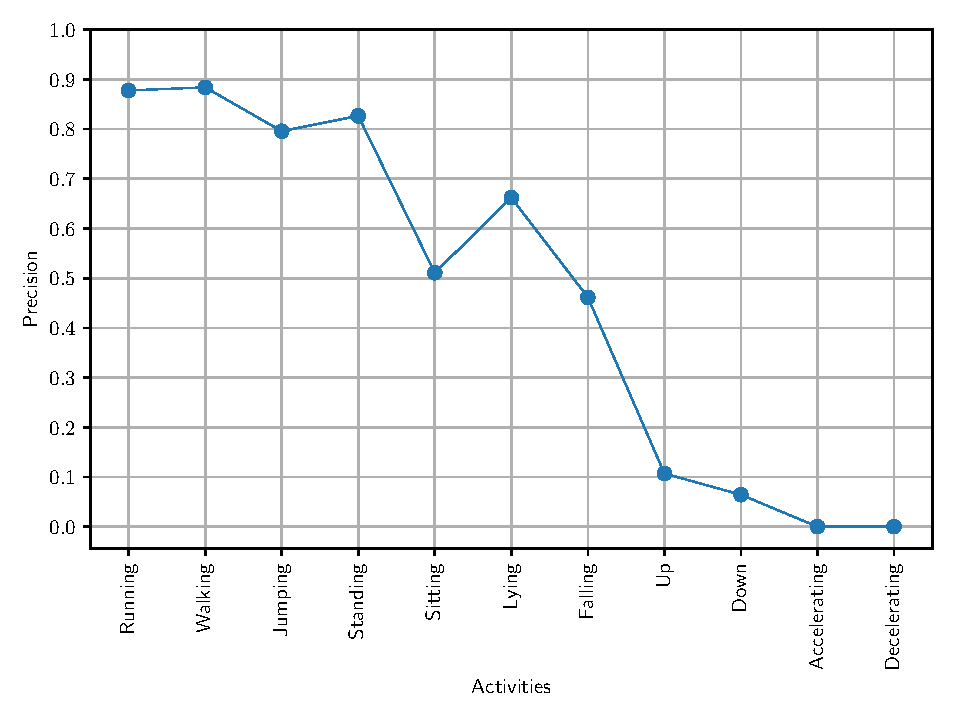
\includegraphics[scale=0.55]{precision.pdf}
\caption{}
\label{fig:precision}
\end{figure}

\begin{figure}
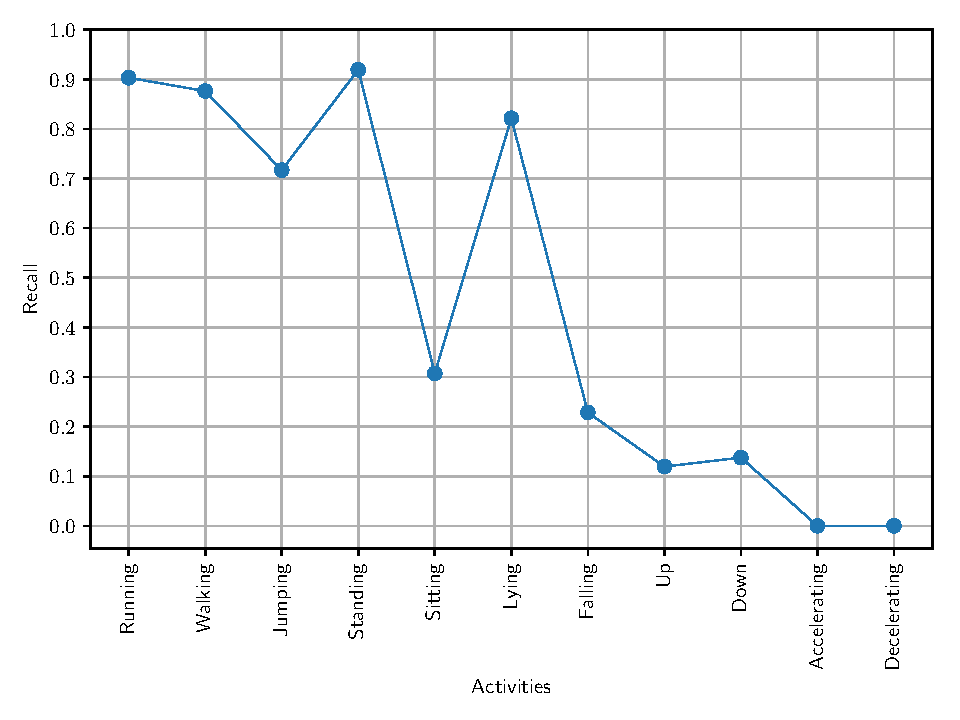
\includegraphics[scale=0.55]{recall.pdf}
\caption{}
\label{fig:recall}
\end{figure}

\red{This section should take max half a page.}

\MR{In many papers, here you find a summary of what done. It is basically an abstract where instead of using the present tense you use the past participle, as you refer to something that you have already developed in the previous sections. While I did it myself in the past, I now find it rather useless.}\\ 

\MR{\textbf{What I would like to see here is:} 1) a very short summary of what done, 2) some (possibly) intelligent observations on the relevance and {\it applicability} of your algorithms / findings, 3) what is still missing, and can be done in the future to extend your work. The idea is that this section should be {\it useful} and not just a repetition of the abstract (just \mbox{re-phrased} and written using a different tense...).}\\

\MR{\textbf{Moreover:} being a project report, I would also like to see a specific paragraph specifying: 1) what you have learned, and 2) any difficulties you may have encountered.}
